\documentclass[11pt,a4paper]{article}

\usepackage[utf8]{inputenc}
\usepackage[T1]{fontenc}
\usepackage[margin=0.95in]{geometry}
\usepackage{amsmath,amssymb,amsfonts,amsthm}
\usepackage{booktabs}
\usepackage{longtable}
\usepackage{array}
\usepackage{graphicx}
\usepackage{float}
\usepackage{xcolor}
\usepackage{hyperref}
\usepackage{fancyhdr}
\usepackage{titlesec}
\usepackage{caption}

\definecolor{navy}{RGB}{24,58,108}
\definecolor{darkred}{RGB}{178,34,34}
\definecolor{darkgreen}{RGB}{34,120,65}
\definecolor{slate}{RGB}{65,75,86}

\hypersetup{
    colorlinks=true,
    linkcolor=navy,
    citecolor=navy,
    urlcolor=navy,
    pdftitle={Institutional Market Risk Modelling, Backtesting and Derivatives Stress-Testing Technical Whitepaper},
    pdfauthor={Mukund Ankit}
}

\pagestyle{fancy}
\fancyhf{}
\fancyhead[L]{\small\textcolor{slate}{\textit{Market Risk Modelling, Backtesting \& Derivatives Framework}}}
\fancyhead[R]{\small\textcolor{slate}{\textit{Model Development \& Validation Whitepaper}}}
\fancyfoot[C]{\small\thepage}
\renewcommand{\headrulewidth}{0.4pt}

\titleformat{\section}{\large\bfseries\color{navy}}{\thesection}{1em}{}[\titlerule]
\titleformat{\subsection}{\normalsize\bfseries\color{navy}}{\thesubsection}{0.8em}{}
\titleformat{\subsubsection}{\normalsize\itshape\color{slate}}{\thesubsubsection}{0.8em}{}

\newtheorem{proposition}{Proposition}[section]
\newtheorem{definition}{Definition}[section]

\title{
    \vspace{-1.2cm}
    \textbf{\LARGE\color{navy} Institutional Market Risk Modelling, Backtesting and Derivatives Stress-Testing Technical Whitepaper}\\[0.35cm]
    \large A Step-by-Step Quantitative Model Development and Validation Document\\
    for a USD 10,000,000 Multi-Asset Macro Trading Desk (Python + C++17 Kernel)
}
\author{\textbf{Mukund Ankit}\\Quantitative Risk Engineering \& Model Validation}
\date{November 2026 $\cdot$ Version 1.0.0}

\begin{document}

\maketitle
\thispagestyle{empty}

\begin{abstract}
\noindent This technical whitepaper documents the end-to-end mathematical formulation, software engineering architecture, empirical calibration, out-of-sample statistical backtesting, and non-linear derivatives stress testing of a multi-asset market risk engine built for a \textbf{USD 10,000,000 Macro Trading Desk} (\texttt{SPY} 30\%, \texttt{AAPL} 20\%, \texttt{TLT} 30\%, \texttt{GLD} 20\%). Operating under a Chief Risk Officer (CRO) governance mandate of \textbf{1-Day 99\% Value-at-Risk ($\text{VaR}_{0.99}$) $\le$ USD 200,000} and \textbf{1-Day 99\% Expected Shortfall ($\text{ES}_{0.99}$) $\le$ USD 280,000}, the document traces the chronological progression of the modelling lifecycle across five distinct phases. First, \textbf{Phase 0} establishes strict point-in-time ($\mathcal{F}_{t-1}$) data hygiene, verifies unit-root non-stationarity in price levels versus $I(0)$ stationarity in daily returns via Augmented Dickey-Fuller tests ($p < 10^{-15}$), proves that portfolio returns exhibit severe leptokurtosis ($K = 9.21 > 3.0$, with $>3\sigma$ tail losses occurring $6.35\times$ more frequently than under a Gaussian benchmark), and diagnoses the 2020 versus 2022 stock--bond correlation regime flip ($\hat{\rho}_{\text{SPY,TLT}}$ shifting from $-0.71$ to $+0.48$). Second, \textbf{Phase 1} implements seven baseline VaR and ES estimators (Plain Historical Simulation with bootstrap standard errors, Parametric Normal, Lognormal, MLE Student-$t$, Cornish-Fisher, and Cholesky Monte Carlo), proves analytically why VaR violates subadditivity on discrete credit payoffs while ES remains coherent, and builds an exact Euler Component/Marginal VaR pre-trade sizer for \texttt{TSLA}. Third, \textbf{Phase 2} diagnoses the 250-day ``Ghost Effect'' plateau in equally weighted rolling windows and upgrades the engine with RiskMetrics EWMA ($\lambda=0.94$), Bollerslev $\text{GARCH}(1,1)$ (Normal and Student-$t$), Age-Weighted Historical Simulation (BRW), and Hull-White Volatility-Weighted Historical Simulation (VWHS). Fourth, \textbf{Phase 3} subjects all seven estimators to a 1,500-day out-of-sample backtest (2020--2025) across the Basel Traffic Light framework, Kupiec POF unconditional coverage ($LR_{UC}$), and Christoffersen Markov independence and conditional coverage ($LR_{IND}, LR_{CC}$), proving that while Plain HS fails independence due to clustered exceptions ($n_{11}=2, p_{IND}=0.040$), Hull-White VWHS ($p_{CC}=0.604$) and $\text{GARCH}(1,1)$ Student-$t$ ($p_{CC}=0.170$) pass all validation criteria with zero consecutive clustering. Finally, \textbf{Phase 4} deploys a compiled C++17 Black-Scholes-Merton kernel to invert \texttt{SPY} option implied volatility surfaces, compute analytical Greeks ($\Delta, \Gamma, \mathcal{V}, \Theta$), expose the catastrophic blindness of linear Delta-Normal VaR on delta-neutral option straddles ($\$0$ vs.\ $\$31,305$), and evaluate protective put hedges across 2020/2022 historical crisis replays and a $5 \times 5$ Spot $\times$ Volatility stress grid.
\end{abstract}

\tableofcontents
\newpage

% ==============================================================================
\section{Trading Desk Governance Mandate, System Architecture and Point-in-Time Data Engineering}
% ==============================================================================

\subsection{Institutional Trading Desk Mandate and Risk Governance Limits}

Quantitative risk management within an institutional multi-asset trading operation exists to enforce capital allocation discipline, size pre-trade exposures, and preserve solvency across tranquil and stressed market regimes. Rather than treating risk metrics as abstract statistical outputs, the risk engine documented in this whitepaper governs a \textbf{USD 10,000,000 Multi-Asset Macro Trading Desk} configured in \texttt{config/portfolio.yaml}. The desk holds a strategic cross-asset allocation designed to capture broad equity market beta, concentrated single-stock growth exposure, sovereign fixed-income duration, and safe-haven commodity protection.

Specifically, the USD 10,000,000 notional capital ($V_0 = \$10,000,000$) is allocated across four liquid exchange-traded instruments: \textbf{30\% in the S\&P 500 Index ETF (\texttt{SPY}, USD 3,000,000)} representing core US equity market beta; \textbf{20\% in Apple Inc.\ (\texttt{AAPL}, USD 2,000,000)} representing concentrated single-name technology risk; \textbf{30\% in the iShares 20+ Year US Treasury Bond ETF (\texttt{TLT}, USD 3,000,000)} introducing long-duration sovereign interest-rate sensitivity and potential equity-bond diversification; and \textbf{20\% in the SPDR Gold Trust (\texttt{GLD}, USD 2,000,000)} providing inflation and tail-crisis hedging behavior.

\begin{table}[H]
\centering
\caption{Baseline USD 10,000,000 Multi-Asset Macro Trading Desk Allocation (\texttt{config/portfolio.yaml})}
\small
\begin{tabular}{llrrl}
\toprule
\textbf{Ticker} & \textbf{Asset Class \& Role} & \textbf{Weight ($w_i$)} & \textbf{Notional ($V_i$)} & \textbf{Primary Risk Factor Sensitivity} \\
\midrule
\texttt{SPY} & US Large-Cap Equities (S\&P 500 ETF) & 30.0\% & \$3,000,000 & Broad US Equity Beta \& Implied Vol (VIX) \\
\texttt{AAPL} & US Tech Single-Stock Equity (Apple) & 20.0\% & \$2,000,000 & Equity Beta + Idiosyncratic Tail Risk \\
\texttt{TLT} & US Long-Duration Sovereign Bonds & 30.0\% & \$3,000,000 & Long-End Treasury Yield Duration \\
\texttt{GLD} & Precious Metals / Safe-Haven Gold & 20.0\% & \$2,000,000 & Real Interest Rates, USD \& Crisis Hedge \\
\midrule
\textbf{Total} & \textbf{Multi-Asset Macro Book} & \textbf{100.0\%} & \textbf{\$10,000,000} & \textbf{Cross-Asset Vol \& Correlation Regimes} \\
\bottomrule
\end{tabular}
\end{table}

The Chief Risk Officer (CRO) enforces two binding daily governance limits over a 1-trading-day holding period ($\Delta t = 1\text{ day}$) at the $\alpha = 99\%$ confidence level, in alignment with the Basel Committee on Banking Supervision (BCBS) Market Risk Framework:
\begin{enumerate}
    \item \textbf{1-Day 99\% Value-at-Risk (VaR) Limit:} $\text{VaR}_{0.99, 1\text{d}} \le \text{USD } 200,000$ ($2.00\%$ of portfolio Net Asset Value).
    \item \textbf{1-Day 99\% Expected Shortfall (ES) Limit:} $\text{ES}_{0.99, 1\text{d}} \le \text{USD } 280,000$ ($2.80\%$ of portfolio Net Asset Value).
\end{enumerate}

\subsection{Hybrid Python and C++17 Quantitative System Architecture}

A central architectural design principle of this framework is the separation of high-level econometric orchestration, data engineering, and visualization in \textbf{Python 3.13} from compute-intensive numerical pricing, root-finding, and time-series recursion in a \textbf{compiled C++17 shared-library kernel} (\texttt{src/cpp/quant\_core.cpp} bound via \texttt{src/cpp\_kernel.py}). In institutional quantitative libraries, research analysts inspect results through interactive notebooks, but inner-loop calculations---such as repricing an option book across $M = 20,000$ joint spot-volatility Monte Carlo scenarios or iterating exponentially weighted moving average (EWMA) variance recursions---must execute at native compiled speed.

\begin{table}[H]
\centering
\caption{Modular Codebase Architecture Across Python and C++17 Layers}
\small
\begin{tabular}{llp{7.8cm}}
\toprule
\textbf{Layer} & \textbf{Module / Notebook} & \textbf{Mathematical \& Engineering Scope} \\
\midrule
Governance Config & \texttt{config/portfolio.yaml} & Portfolio weights, \$10M notional, CRO VaR/ES limits, lookback windows, decay factors, and stress grids. \\
C++17 Kernel & \texttt{src/cpp/quant\_core.cpp} & Compiled with \texttt{-O3 -std=c++17 -shared -fPIC}; BSM pricing, analytical Greeks, safeguarded Newton-Bisection IV solver, vectorized MC revaluation, and EWMA recursion. \\
Data Pipeline & \texttt{src/data\_loader.py} & Total-return adjusted closes, NYSE calendar alignment, Parquet caching, and strict $\mathcal{F}_{t-1}$ point-in-time slicing. \\
Phase 0 (EDA) & \texttt{src/eda\_diagnostics.py} & ADF unit-root tests, Jarque-Bera tests, higher moments, Q-Q coordinates, and rolling regime correlations. \\
Phase 1 (Crawl) & \texttt{src/var\_estimators.py} & Plain HS (bootstrap SE), Normal, Lognormal, MLE Student-$t$, Cornish-Fisher, Cholesky MC, subadditivity proofs, and \texttt{TSLA} Marginal VaR trade sizer. \\
Phase 2 (Walk) & \texttt{src/volatility\_models.py} & Ghost-effect diagnosis, RiskMetrics EWMA ($\lambda=0.94$), $\text{GARCH}(1,1)$ (Normal \& Student-$t$), Age-Weighted HS, and Hull-White Volatility-Weighted HS. \\
Phase 3 (Walk+) & \texttt{src/backtesting.py} & 1,500-day OOS backtest, Basel Traffic Light zones, Kupiec POF ($LR_{UC}$), and Christoffersen Markov tests ($LR_{IND}, LR_{CC}$). \\
Phase 4 (Run) & \texttt{src/derivatives\_stress.py} & \texttt{SPY} option skew, analytical Greeks, Delta-Normal vs.\ Delta-Gamma-Vega vs.\ Full Revaluation MC, 2020/2022 crisis replays, and $5\times 5$ stress grids. \\
Unit Verification & \texttt{tests/test\_risk\_engine.py} & Automated \texttt{pytest} suite verifying closed-form identities, put-call parity, and backtest discrimination. \\
\bottomrule
\end{tabular}
\end{table}

\subsection{Data Hygiene Rules, Return Transformations and Zero Look-Ahead Slicing}

To guarantee institutional data integrity across the 11-year historical sample spanning \textbf{January 1, 2015 to December 31, 2025} ($N = 2,797$ aligned daily return observations across \texttt{SPY}, \texttt{AAPL}, \texttt{TLT}, \texttt{GLD}, \texttt{TSLA}, and the Cboe Volatility Index \texttt{VIX}), \texttt{src/data\_loader.py} enforces three mandatory hygiene rules: (i) extraction of \textbf{Total-Return Adjusted Close} prices so stock splits and dividend payouts never appear as artificial single-day price crashes; (ii) inner-joining all series on NYSE trading dates with at most 1 consecutive day of forward-filling; and (iii) strict \textbf{point-in-time slicing} ($\mathcal{F}_{t-1} = \{r_1, \dots, r_{t-1}\}$) via \texttt{slice\_point\_in\_time}, guaranteeing zero look-ahead bias.

For each asset $i \in \{1, \dots, N\}$, the pipeline computes both daily \textbf{arithmetic returns} $r_{i,t}$ and \textbf{geometric log returns} $R_{i,t}$:
\begin{equation}
r_{i,t} = \frac{P_{i,t} - P_{i,t-1}}{P_{i,t-1}}, \qquad R_{i,t} = \ln\left(\frac{P_{i,t}}{P_{i,t-1}}\right) = \ln(1 + r_{i,t})
\end{equation}
Geometric log returns aggregate additively across time ($\sum_{t=1}^T R_{i,t} = \ln(P_{i,T}/P_{i,0})$), whereas arithmetic returns aggregate linearly across the cross-section of portfolio weights $\mathbf{w} = (w_1, \dots, w_N)^\top$:
\begin{equation}
r_{p,t} = \sum_{i=1}^{N} w_i r_{i,t} = \mathbf{w}^\top \mathbf{r}_t, \qquad \text{P\&L}_t = V_0 r_{p,t}, \qquad L_t = -\text{P\&L}_t = -V_0 r_{p,t}
\end{equation}
where $L_t$ denotes the daily \textbf{portfolio dollar loss}. Both identities are verified across all 2,797 trading days in \texttt{00\_data\_hygiene\_and\_eda.ipynb}, yielding a maximum temporal log-return additivity error of $7.11 \times 10^{-15}$ and a cross-sectional linearity error of $0.00 \times 10^0$.

% ==============================================================================
\section{Phase 0: Exploratory Data Analysis, Stationarity and Distributional Stylized Facts}
% ==============================================================================

\subsection{Unit Root Testing and Time-Series Stationarity Verification}

Before estimating sample covariance matrices, empirical quantiles, or GARCH conditional variance equations, a quantitative modeller must verify that the underlying time series is covariance-stationary. Applying a risk estimator directly to a non-stationary random walk with drift ($P_t = \mu + P_{t-1} + \varepsilon_t$) yields spurious sample variances that grow linearly with time ($t\sigma_\varepsilon^2$). In \texttt{src/eda\_diagnostics.py}, the \textbf{Augmented Dickey-Fuller (ADF) test} (Dickey and Fuller, 1979) is estimated on both raw price levels ($P_{i,t}$) and daily arithmetic returns ($r_{i,t}$):
\begin{equation}
\Delta Y_t = \alpha + \gamma Y_{t-1} + \sum_{j=1}^{p^*} \delta_j \Delta Y_{t-j} + u_t
\end{equation}
testing the unit-root null hypothesis $\mathcal{H}_0: \gamma = 0$ ($I(1)$ non-stationary) against the stationary alternative $\mathcal{H}_1: \gamma < 0$ ($I(0)$ stationary), with lag length $p^*$ selected via the Akaike Information Criterion (AIC).

\begin{table}[H]
\centering
\caption{Augmented Dickey-Fuller (ADF) Stationarity Verification (\texttt{00\_data\_hygiene\_and\_eda.ipynb})}
\small
\begin{tabular}{llrrrrrc}
\toprule
\textbf{Asset} & \textbf{Tested Series} & \textbf{ADF Stat ($\tau$)} & \textbf{$p$-Value} & \textbf{Lags} & \textbf{1\% Crit} & \textbf{5\% Crit} & \textbf{Stationary (5\%)} \\
\midrule
\texttt{SPY}  & Price Level ($P_t$)  & $-1.7821$ & $3.8936 \times 10^{-1}$ & 28 & $-3.4327$ & $-2.8626$ & \textcolor{darkred}{\textbf{False}} \\
\texttt{SPY}  & Daily Return ($r_t$) & $-10.1509$ & $7.9565 \times 10^{-18}$ & 27 & $-3.4327$ & $-2.8626$ & \textcolor{darkgreen}{\textbf{True}} \\
\texttt{AAPL} & Price Level ($P_t$)  & $-0.4297$ & $9.0503 \times 10^{-1}$ & 9  & $-3.4327$ & $-2.8626$ & \textcolor{darkred}{\textbf{False}} \\
\texttt{AAPL} & Daily Return ($r_t$) & $-17.9573$ & $2.8250 \times 10^{-30}$ & 11 & $-3.4327$ & $-2.8626$ & \textcolor{darkgreen}{\textbf{True}} \\
\texttt{TLT}  & Price Level ($P_t$)  & $-0.9157$ & $7.8276 \times 10^{-1}$ & 28 & $-3.4327$ & $-2.8626$ & \textcolor{darkred}{\textbf{False}} \\
\texttt{TLT}  & Daily Return ($r_t$) & $-9.6586$  & $1.3731 \times 10^{-16}$ & 27 & $-3.4327$ & $-2.8626$ & \textcolor{darkgreen}{\textbf{True}} \\
\texttt{GLD}  & Price Level ($P_t$)  & $-1.1812$ & $6.8162 \times 10^{-1}$ & 28 & $-3.4327$ & $-2.8626$ & \textcolor{darkred}{\textbf{False}} \\
\texttt{GLD}  & Daily Return ($r_t$) & $-13.9086$ & $5.5648 \times 10^{-26}$ & 12 & $-3.4327$ & $-2.8626$ & \textcolor{darkgreen}{\textbf{True}} \\
\bottomrule
\end{tabular}
\end{table}

As shown in Table 3, every raw price series fails to reject the unit-root null hypothesis ($p \in [0.389, 0.905]$), whereas every daily return series rejects the unit-root null at $p < 10^{-15}$, confirming that return transformations produce stationary $I(0)$ inputs.

\subsection{Higher-Moment Stylized Facts: Leptokurtosis, Negative Skewness and Normality Rejection}

Under a univariate Gaussian assumption $r_t \sim \mathcal{N}(\mu, \sigma^2)$, skewness is $S = 0$, total kurtosis is $K = 3$ (excess kurtosis $K_{\text{ex}} = K - 3 = 0$), and the two-sided probability of observing a daily shock exceeding three standard deviations ($|z_t| > 3.0$) is $0.270\%$. To test Gaussianity empirically, \texttt{src/eda\_diagnostics.py} computes the sample moments, the $>3\sigma$ exceedance frequency ratio, and the \textbf{Jarque-Bera (JB) statistic}:
\begin{equation}
\text{JB} = \frac{N}{6}\left(\hat{S}^2 + \frac{\hat{K}_{\text{ex}}^2}{4}\right) \xrightarrow{d} \chi^2_2 \quad \text{under } \mathcal{H}_0: r_t \sim \mathcal{N}(\mu, \sigma^2)
\end{equation}

\begin{table}[H]
\centering
\caption{Distributional Stylized Facts Across Assets and the \$10M Portfolio (2015--2025)}
\footnotesize
\begin{tabular}{lrrrrrrrrr}
\toprule
\textbf{Asset / Book} & \textbf{Ann.\ Ret} & \textbf{Ann.\ Vol} & \textbf{Skew ($\hat{S}$)} & \textbf{Ex.\ Kurt} & \textbf{Tot.\ Kurt} & \textbf{Min / Max Daily} & \textbf{$>3\sigma$ Freq} & \textbf{Tail Ratio} & \textbf{JB Stat} \\
\midrule
\texttt{SPY} & 5.25\% & 16.30\% & $-0.532$ & 16.927 & 19.927 & $-11.89\% / +10.06\%$ & 1.573\% & \textbf{5.82x} & 33,408.0 \\
\texttt{AAPL} & 12.17\% & 25.46\% & $-0.584$ & 13.839 & 16.839 & $-17.90\% / +14.49\%$ & 1.251\% & \textbf{4.63x} & 22,401.4 \\
\texttt{TLT} & $-2.75\%$ & 14.05\% & $-0.267$ & 8.560 & 11.560 & $-7.69\% / +6.49\%$ & 1.251\% & \textbf{4.63x} & 8,540.2 \\
\texttt{GLD} & 6.42\% & 12.76\% & $+0.792$ & 10.180 & 13.180 & $-3.61\% / +9.24\%$ & 1.215\% & \textbf{4.50x} & 12,326.8 \\
\midrule
\textbf{PORTFOLIO} & \textbf{4.47\%} & \textbf{9.92\%} & \textbf{$-0.444$} & \textbf{6.208} & \textbf{9.208} & \textbf{$-5.63\% / +3.45\%$} & \textbf{1.716\%} & \textbf{6.35x} & \textbf{4,566.3} \\
\bottomrule
\end{tabular}
\end{table}

Table 4 and Figure 1 demonstrate that the aggregate USD 10,000,000 portfolio exhibits negative skewness ($\hat{S} = -0.444$) and substantial leptokurtosis ($\hat{K}_{\text{ex}} = 6.208$, total kurtosis $\hat{K} = 9.208 > 3.0$). Extreme $>3\sigma$ tail events occur on $1.716\%$ of trading days---\textbf{$6.35\times$ more frequently} than predicted by a Normal distribution---and the Jarque-Bera test ($4,566.3 > 5.991$) rejects Gaussianity at $p = 0.0$.

\begin{figure}[H]
\centering
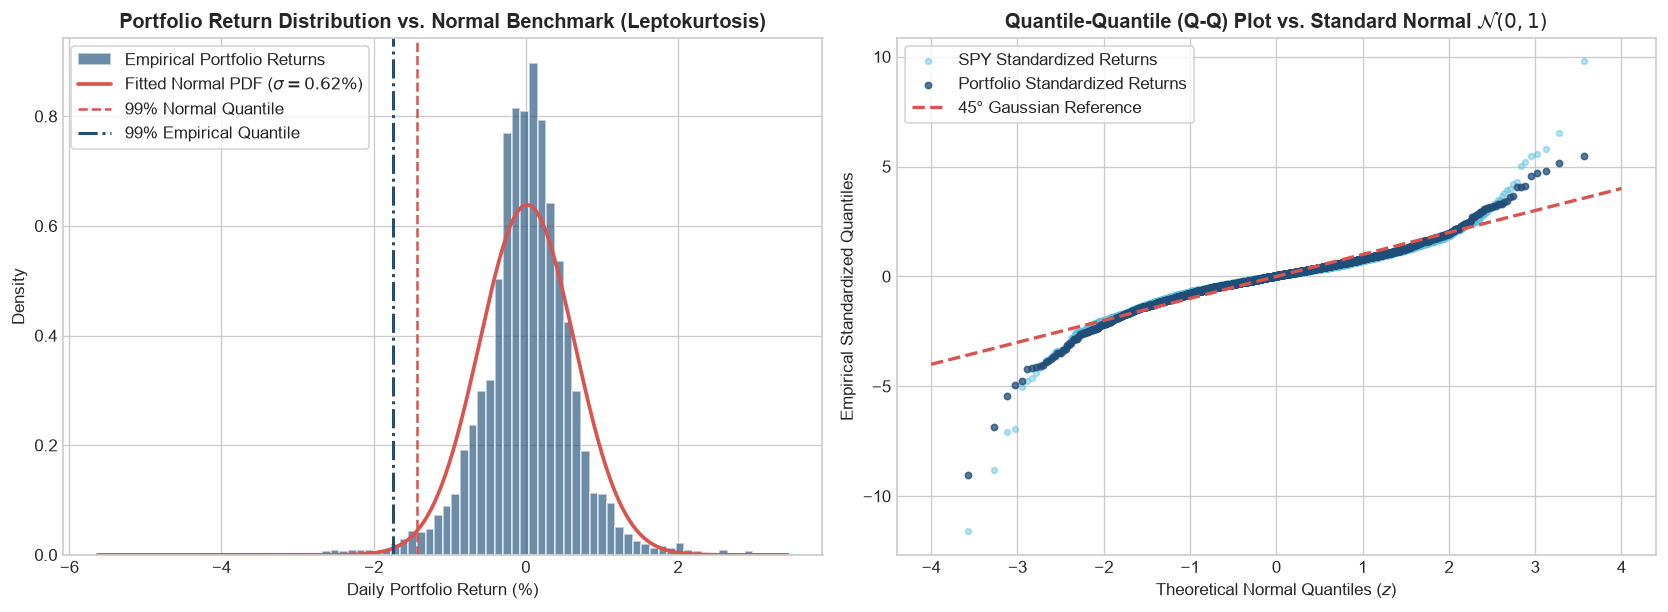
\includegraphics[width=0.98\textwidth]{figures/fig01_qq_and_distribution.png}
\caption{Left: Empirical daily portfolio return histogram versus fitted Gaussian density ($\sigma_p = 0.62\%$), illustrating the sharper peak and heavier left tail of empirical returns. Right: Normal Quantile-Quantile (Q-Q) plot showing pronounced S-shaped tail departure from $\mathcal{N}(0,1)$.}
\end{figure}

\subsection{Volatility Clustering and the 2020 vs.\ 2022 Stock--Bond Correlation Regime Flip}

To examine how risk parameters evolve across macroeconomic cycles, Figure 2 plots the 20-day rolling annualized realized volatility alongside the Cboe VIX index (top panel) and the 60-day rolling correlation $\hat{\rho}_{60\text{d}, t}(\text{SPY}, \text{TLT})$ between equities and long-term Treasuries (bottom panel).

\begin{table}[H]
\centering
\caption{Cross-Asset Volatility and Equity--Treasury Correlation Across Macro Regimes}
\small
\begin{tabular}{llrrrr}
\toprule
\textbf{Macro Market Regime} & \textbf{Calendar Window} & \textbf{Days} & \textbf{$\hat{\rho}(\text{SPY},\text{TLT})$} & \textbf{SPY Vol} & \textbf{TLT Vol} \\
\midrule
Full Sample (2015--2025) & 2015-01-01 to 2025-12-31 & 2,797 & $-0.2611$ & 16.30\% & 14.05\% \\
2017 Low-Volatility Calm & 2017-01-01 to 2017-12-31 & 253 & $-0.4288$ & 9.32\% & 8.66\% \\
2020 COVID-19 Crisis (Q1--Q2) & 2020-02-01 to 2020-05-31 & 84 & \textcolor{darkgreen}{\textbf{$-0.7093$}} & \textbf{51.49\%} & \textbf{39.76\%} \\
2022 Inflation \& Rate-Hike Bear & 2022-01-01 to 2022-12-31 & 253 & \textcolor{darkred}{\textbf{$+0.4829$}} & 21.00\% & 20.74\% \\
2023--2025 Post-Hike Regime & 2023-01-01 to 2025-12-31 & 761 & $-0.1261$ & 14.04\% & 11.20\% \\
\bottomrule
\end{tabular}
\end{table}

\begin{figure}[H]
\centering
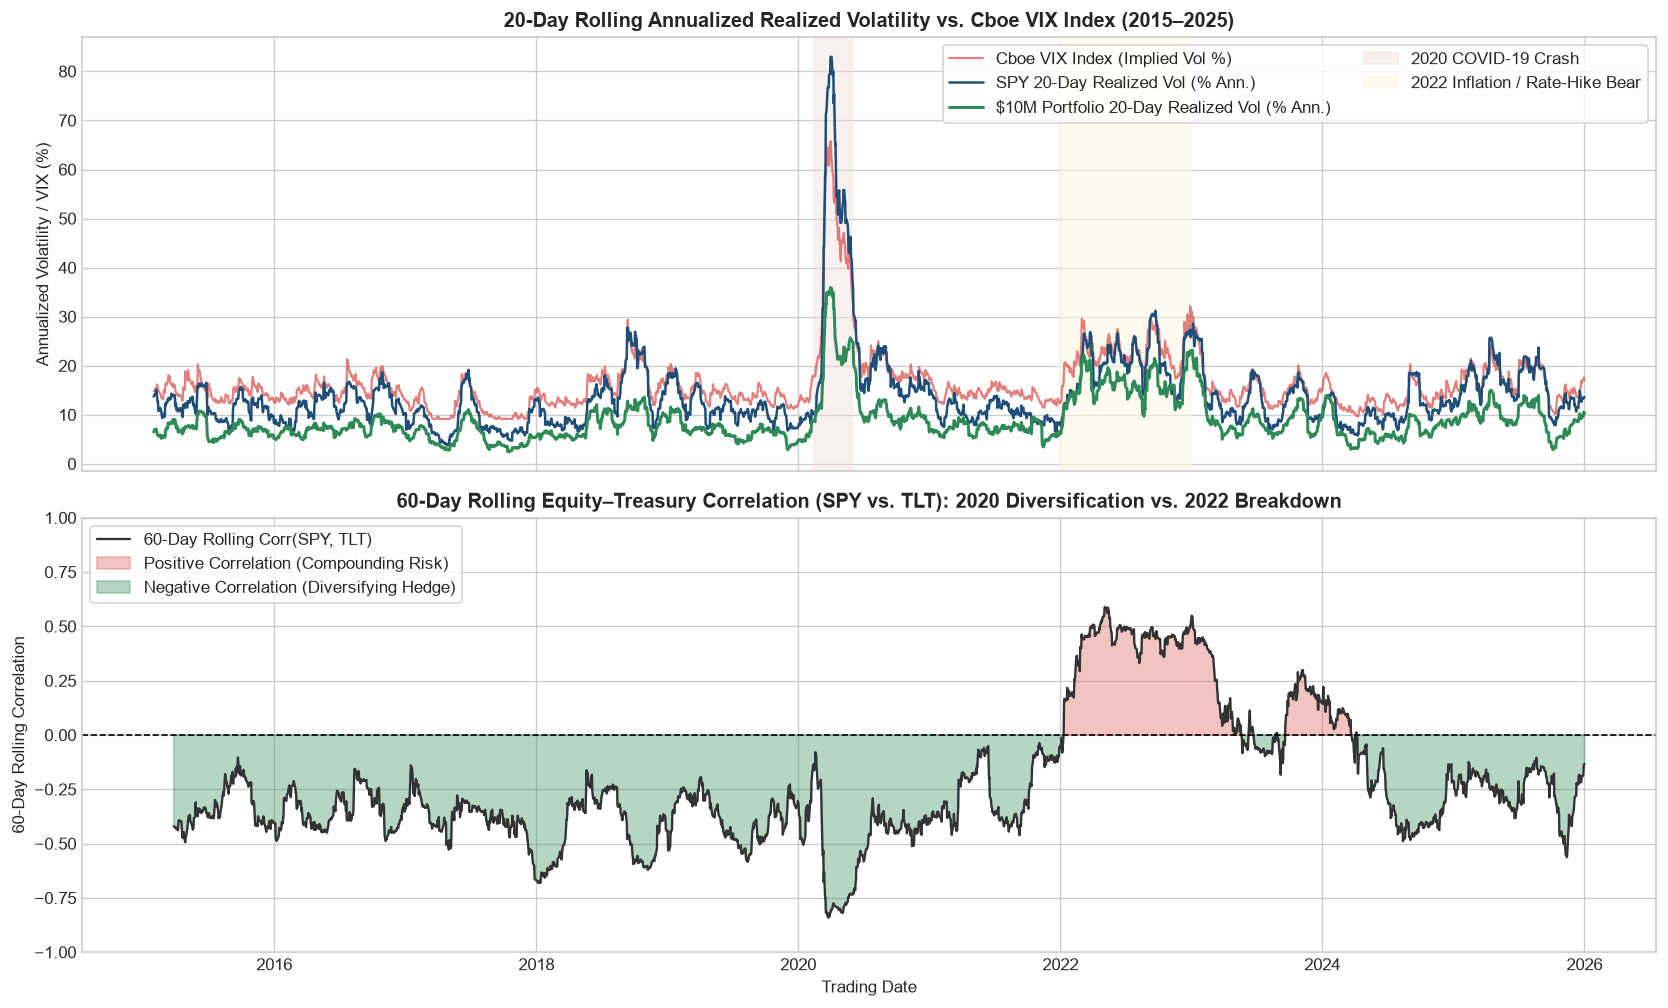
\includegraphics[width=0.98\textwidth]{figures/fig02_volatility_and_correlation_regimes.png}
\caption{Top: 20-day rolling annualized volatility of \texttt{SPY} and the \$10M portfolio alongside the Cboe VIX index. Bottom: 60-day rolling \texttt{SPY}--\texttt{TLT} correlation, highlighting the shift from negative (diversifying) in Q1 2020 ($\hat{\rho} = -0.71$) to positive (compounding losses) in 2022 ($\hat{\rho} = +0.48$).}
\end{figure}

\noindent\textbf{Modeller's Progression Decision (Phase 0 $\rightarrow$ Phase 1):} Because portfolio returns reject normality ($K = 9.21, S = -0.44$) and cross-asset correlations shift dramatically across regimes, static Gaussian VaR will systematically understate tail risk. Phase 1 therefore builds non-parametric Historical Simulation, fat-tailed parametric specifications (MLE Student-$t$ and Cornish-Fisher), and Cholesky Monte Carlo simulation, while linking risk attribution to CRO limit governance.

% ==============================================================================
\section{Phase 1 (Crawl): Baseline VaR \& Expected Shortfall Engine, Coherence Proofs and Pre-Trade Sizing}
% ==============================================================================

\subsection{Mathematical Formulation of Baseline VaR and Expected Shortfall Estimators}

For daily portfolio dollar loss $L_t = -V_0 r_{p,t}$ with distribution $F_L(\ell) = \mathbb{P}(L_t \le \ell)$ and confidence level $\alpha \in \{0.95, 0.99\}$, \textbf{Value-at-Risk ($\text{VaR}_\alpha$)} and \textbf{Expected Shortfall ($\text{ES}_\alpha$)} (Acerbi and Tasche, 2002) are defined as:
\begin{equation}
\text{VaR}_\alpha(L) = \inf\{\ell \in \mathbb{R} : F_L(\ell) \ge \alpha\}, \qquad \text{ES}_\alpha(L) = \mathbb{E}\left[L_t \;\middle|\; L_t \ge \text{VaR}_\alpha(L)\right] = \frac{1}{1-\alpha}\int_{\alpha}^{1} \text{VaR}_u(L)\,du
\end{equation}

In \texttt{src/var\_estimators.py}, six baseline methodologies are implemented:
\begin{enumerate}
    \item \textbf{Plain Historical Simulation ($n=250$ and $n=500$ days + Bootstrap SE):} Sorting the $n$ historical dollar losses in descending order $L_{(1)} \ge L_{(2)} \ge \dots \ge L_{(n)}$, $\text{VaR}_\alpha^{\text{HS}} = L_{(k)}$ where $k = \lfloor (1-\alpha)n \rfloor + 1$, and $\text{ES}_\alpha^{\text{HS}} = \frac{1}{k}\sum_{j=1}^k L_{(j)}$, accompanied by a 500-replication non-parametric bootstrap standard error $\text{SE}_{\text{boot}}(\text{VaR}_\alpha^{\text{HS}})$.
    \item \textbf{Parametric Variance-Covariance (Normal):} With sample portfolio mean $\hat{\mu}_p = \mathbf{w}^\top\hat{\boldsymbol{\mu}}$ and volatility $\hat{\sigma}_p = \sqrt{\mathbf{w}^\top\hat{\mathbf{\Sigma}}\mathbf{w}}$:
    \begin{equation}
    \text{VaR}_\alpha^{\text{Norm}} = V_0\left(-\hat{\mu}_p + \hat{\sigma}_p z_\alpha\right), \qquad \text{ES}_\alpha^{\text{Norm}} = V_0\left(-\hat{\mu}_p + \hat{\sigma}_p \frac{\phi(z_\alpha)}{1-\alpha}\right)
    \end{equation}
    \item \textbf{Parametric Lognormal:} Modeling geometric log returns $R_{p,t} \sim \mathcal{N}(\hat{\mu}_R, \hat{\sigma}_R^2)$:
    \begin{equation}
    \text{VaR}_\alpha^{\text{Lognorm}} = V_0\left(1 - \exp(\hat{\mu}_R - \hat{\sigma}_R z_\alpha)\right), \qquad \text{ES}_\alpha^{\text{Lognorm}} = V_0\left(1 - \frac{\exp(\hat{\mu}_R + \frac{1}{2}\hat{\sigma}_R^2)\Phi(-z_\alpha - \hat{\sigma}_R)}{1-\alpha}\right)
    \end{equation}
    \item \textbf{Parametric Student-$t$ (MLE Degrees of Freedom $\hat{\nu}$):} Fitting $\hat{\nu}$ via Maximum Likelihood and scaling dispersion by $\hat{\sigma}_{\text{scale}} = \hat{\sigma}_p\sqrt{(\hat{\nu}-2)/\hat{\nu}}$:
    \begin{equation}
    \text{VaR}_\alpha^{t} = V_0\left(-\hat{\mu}_p + \hat{\sigma}_{\text{scale}}\,t_{\hat{\nu},\alpha}\right), \qquad \text{ES}_\alpha^{t} = V_0\left(-\hat{\mu}_p + \hat{\sigma}_{\text{scale}}\frac{g_{\hat{\nu}}(t_{\hat{\nu},\alpha})}{1-\alpha}\left(\frac{\hat{\nu} + t_{\hat{\nu},\alpha}^2}{\hat{\nu}-1}\right)\right)
    \end{equation}
    \item \textbf{Cornish-Fisher Semi-Parametric Expansion:} Injecting sample loss skewness $\hat{S}_L = -\hat{S}_r$ and excess kurtosis $\hat{K}_{\text{ex}}$ into the standard normal quantile $z_\alpha$ (Cornish and Fisher, 1938):
    \begin{equation}
    z_{\text{CF}}(\alpha) = z_\alpha + \frac{1}{6}(z_\alpha^2 - 1)\hat{S}_L + \frac{1}{24}(z_\alpha^3 - 3z_\alpha)\hat{K}_{\text{ex}} - \frac{1}{36}(2z_\alpha^3 - 5z_\alpha)\hat{S}_L^2
    \end{equation}
    \item \textbf{Cholesky Monte Carlo Simulation ($M = 10,000$):} Factorizing $\hat{\mathbf{\Sigma}} = \mathbf{L}\mathbf{L}^\top$, drawing antithetic standard normal vectors $\mathbf{Z}^{(m)} \sim \mathcal{N}(\mathbf{0}, \mathbf{I}_N)$, simulating $\mathbf{r}^{(m)} = \hat{\boldsymbol{\mu}} + \mathbf{L}\mathbf{Z}^{(m)}$, and extracting empirical tail quantiles.
\end{enumerate}

\subsection{Empirical Comparison of Phase 1 Estimators and CRO Limit Governance}

\begin{table}[H]
\centering
\caption{Phase 1 Baseline 1-Day VaR and Expected Shortfall Dashboard (\texttt{01\_baseline\_var\_and\_es.ipynb})}
\footnotesize
\begin{tabular}{lcrrrrrc}
\toprule
\textbf{Estimator} & \textbf{Conf.} & \textbf{VaR (USD)} & \textbf{VaR (\%)} & \textbf{ES (USD)} & \textbf{ES (\%)} & \textbf{Boot SE} & \textbf{CRO Limit Status} \\
\midrule
Historical Simulation (250d) & 95\% & \$109,065.89 & 1.09\% & \$135,950.71 & 1.36\% & \$9,587.75 & Within Limit \\
Historical Simulation (500d) & 95\% & \$88,660.47 & 0.89\% & \$119,078.16 & 1.19\% & \$7,364.35 & Within Limit \\
Parametric Normal (Var-Cov) & 95\% & \$107,375.33 & 1.07\% & \$134,340.75 & 1.34\% & --- & Within Limit \\
Parametric Lognormal & 95\% & \$106,957.87 & 1.07\% & \$133,558.42 & 1.34\% & --- & Within Limit \\
Parametric Student-$t$ ($\hat{\nu}=7.3$) & 95\% & \$104,793.56 & 1.05\% & \$142,364.77 & 1.42\% & --- & Within Limit \\
Cornish-Fisher Semi-Parametric & 95\% & \$102,194.62 & 1.02\% & \$134,925.79 & 1.35\% & --- & Within Limit \\
Cholesky Monte Carlo ($M=10,000$) & 95\% & \$105,935.35 & 1.06\% & \$133,964.62 & 1.34\% & --- & Within Limit \\
\midrule
Historical Simulation (250d) & \textbf{99\%} & \textbf{\$158,473.92} & \textbf{1.58\%} & \textbf{\$173,658.09} & \textbf{1.74\%} & \textbf{\$17,724.11} & \textcolor{darkgreen}{\textbf{Within (\$41.5k Buf)}} \\
Historical Simulation (500d) & \textbf{99\%} & \textbf{\$136,136.44} & \textbf{1.36\%} & \textbf{\$156,722.50} & \textbf{1.57\%} & \textbf{\$11,805.83} & \textcolor{darkgreen}{\textbf{Within (\$63.9k Buf)}} \\
Parametric Normal (Var-Cov) & \textbf{99\%} & \textbf{\$151,353.73} & \textbf{1.51\%} & \textbf{\$173,221.56} & \textbf{1.73\%} & --- & \textcolor{darkgreen}{\textbf{Within (\$48.6k Buf)}} \\
Parametric Lognormal & \textbf{99\%} & \textbf{\$150,350.47} & \textbf{1.50\%} & \textbf{\$171,836.34} & \textbf{1.72\%} & --- & \textcolor{darkgreen}{\textbf{Within (\$49.6k Buf)}} \\
Parametric Student-$t$ ($\hat{\nu}=7.3$) & \textbf{99\%} & \textbf{\$164,126.49} & \textbf{1.64\%} & \textbf{\$204,959.07} & \textbf{2.05\%} & --- & \textcolor{darkgreen}{\textbf{Within (\$35.9k Buf)}} \\
Cornish-Fisher Semi-Parametric & \textbf{99\%} & \textbf{\$156,793.80} & \textbf{1.57\%} & \textbf{\$185,878.06} & \textbf{1.86\%} & --- & \textcolor{darkgreen}{\textbf{Within (\$43.2k Buf)}} \\
Cholesky Monte Carlo ($M=10,000$) & \textbf{99\%} & \textbf{\$151,617.06} & \textbf{1.52\%} & \textbf{\$173,973.98} & \textbf{1.74\%} & --- & \textcolor{darkgreen}{\textbf{Within (\$48.4k Buf)}} \\
\bottomrule
\end{tabular}
\end{table}

\begin{figure}[H]
\centering
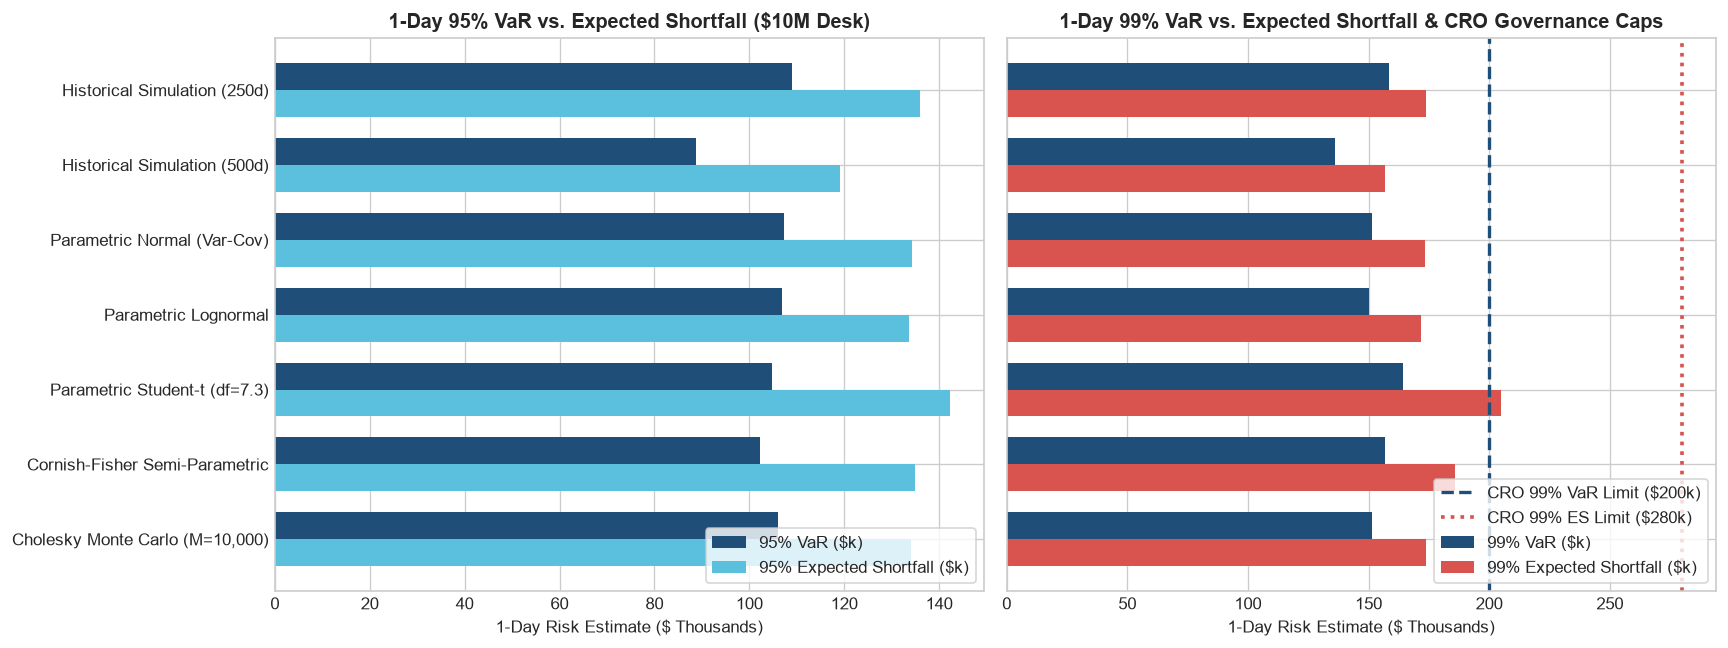
\includegraphics[width=0.98\textwidth]{figures/fig03_phase1_var_es_comparison.png}
\caption{Comparison of 1-Day 95\% (left) and 99\% (right) VaR and Expected Shortfall across all seven Phase 1 estimators benchmarked against the CRO's \$200k VaR and \$280k ES governance caps.}
\end{figure}

As shown in Table 6 and Figure 3, while Gaussian Variance-Covariance ($\text{VaR}_{0.99} = \$151,354$, $\text{ES}_{0.99} = \$173,222$) and Cholesky Monte Carlo ($\text{VaR}_{0.99} = \$151,617$) converge closely, accounting for fat tails via Student-$t$ ($\hat{\nu}=7.3$) raises 1-Day 99\% VaR to \textbf{\$164,126} and increases 1-Day 99\% Expected Shortfall by \textbf{+\$31,738 (+18.3\%) to \$204,959}.

\subsection{Coherence, Portfolio Diversification Benefit and Subadditivity Verification}

Under the axiomatic framework of Artzner et al.\ (1999), a coherent risk measure $\rho(\cdot)$ must satisfy \textbf{subadditivity}: $\rho(L_1 + L_2) \le \rho(L_1) + \rho(L_2)$. On our 4-asset desk, cross-asset diversification saves \textbf{\$88,307.06 (36.8\%)} in 1-Day 99\% Normal VaR ($\$151,353.73$ diversified vs.\ $\$239,660.79$ sum of standalone asset VaRs) and \textbf{\$109,234.81 (40.8\%)} in 1-Day 99\% Historical Simulation VaR ($\$158,473.92$ diversified vs.\ $\$267,708.73$ standalone sum).

\begin{proposition}[Subadditivity Failure of VaR vs.\ Coherence of Expected Shortfall]
Consider two independent corporate bonds $B_1, B_2$, each with face value $\$100,000$ and independent 1-day default probability $p = 0.008$ ($0.8\%$). At confidence level $\alpha = 0.99$ (tail probability $1 - \alpha = 0.01$):
\begin{enumerate}
    \item Because $\mathbb{P}(L_i = \$0) = 0.992 \ge 0.99$, standalone 99\% VaR is $\text{VaR}_{0.99}(L_1) = \text{VaR}_{0.99}(L_2) = \$0$.
    \item For the combined portfolio $L_1 + L_2$, $\mathbb{P}(L_1 + L_2 = \$0) = (0.992)^2 = 0.984064 < 0.99$, so $\text{VaR}_{0.99}(L_1 + L_2) = \$100,000 > \text{VaR}_{0.99}(L_1) + \text{VaR}_{0.99}(L_2) = \$0$, violating subadditivity.
    \item By contrast, 99\% Expected Shortfall satisfies $\text{ES}_{0.99}(L_i) = \frac{0.008(\$100,000)}{0.01} = \$80,000$ and $\text{ES}_{0.99}(L_1 + L_2) = \frac{0.000064(\$200,000) + 0.009936(\$100,000)}{0.01} = \$100,640 \le \$80,000 + \$80,000 = \$160,000$.
\end{enumerate}
\end{proposition}

\subsection{Pre-Trade Marginal and Incremental VaR Sizing for \texttt{TSLA}}

By Euler's Homogeneous Function Theorem, Parametric Normal VaR decomposes additively into asset-level Component VaRs via Marginal VaR per dollar $\Delta\text{VaR}_i = \frac{\partial\text{VaR}_\alpha(\mathbf{x})}{\partial x_i} = -\mu_i + z_\alpha\frac{(\mathbf{\Sigma}\mathbf{x})_i}{\sqrt{\mathbf{x}^\top\mathbf{\Sigma}\mathbf{x}}}$:
\begin{itemize}
    \item \texttt{SPY} (\$3M): Marginal VaR $= \$0.0200/\$$, Component VaR $= \$59,897.88$ ($39.58\%$ of total VaR).
    \item \texttt{AAPL} (\$2M): Marginal VaR $= \$0.0307/\$$, Component VaR $= \$61,493.99$ ($40.63\%$ of total VaR).
    \item \texttt{TLT} (\$3M): Marginal VaR $= \$0.0047/\$$, Component VaR $= \$14,166.09$ ($9.36\%$ of total VaR).
    \item \texttt{GLD} (\$2M): Marginal VaR $= \$0.0079/\$$, Component VaR $= \$15,795.77$ ($10.44\%$ of total VaR).
\end{itemize}

When a portfolio manager proposes adding \texttt{TSLA} ($\Delta\text{VaR}_{\text{TSLA}} = \$0.0397/\$$), solving $\text{VaR}_{0.99}(\mathbf{x}_0 + \Delta x_{\text{TSLA}}\mathbf{e}_{\text{TSLA}}) = \$200,000$ via Brent's root-finding method (\texttt{scipy.optimize.brentq}) caps the maximum allowable \texttt{TSLA} trade at \textbf{USD 961,273.98} under Parametric Normal VaR and \textbf{USD 765,211.44} under Historical Simulation VaR (Figure 4).

\begin{figure}[H]
\centering
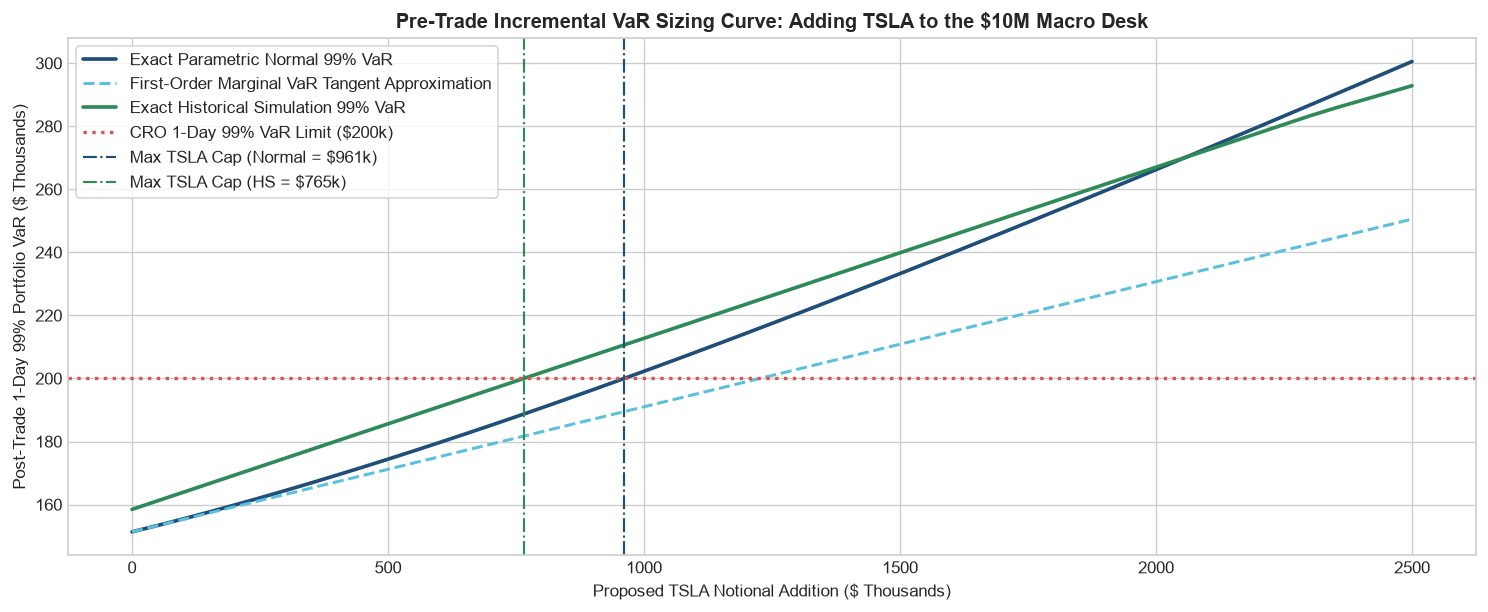
\includegraphics[width=0.95\textwidth]{figures/fig04_tsla_marginal_var_sizing.png}
\caption{Pre-Trade Incremental VaR sizing curve for adding \texttt{TSLA} to the \$10M Macro Desk, comparing exact Parametric Normal VaR, first-order Marginal VaR tangent approximation, and exact Historical Simulation VaR against the CRO's \$200,000 cap.}
\end{figure}

% ==============================================================================
\section{Phase 2 (Walk): Time-Series Volatility Regimes and Dynamic Historical Simulation}
% ==============================================================================

\subsection{Diagnosing the 250-Day ``Ghost Effect'' and Conditional Volatility Models}

Equally weighted $n = 250$-day rolling windows weight every observation in $[t-250, t-1]$ by $1/250$ and drop observation $t-251$ to weight zero. As demonstrated in Figure 5, after the March 2020 COVID-19 crash, Plain 250-day Historical Simulation 99\% VaR jumps to \textbf{\$343,189} and remains trapped on a flat horizontal plateau for exactly 250 trading days before plunging off a cliff in March 2021.

\begin{figure}[H]
\centering
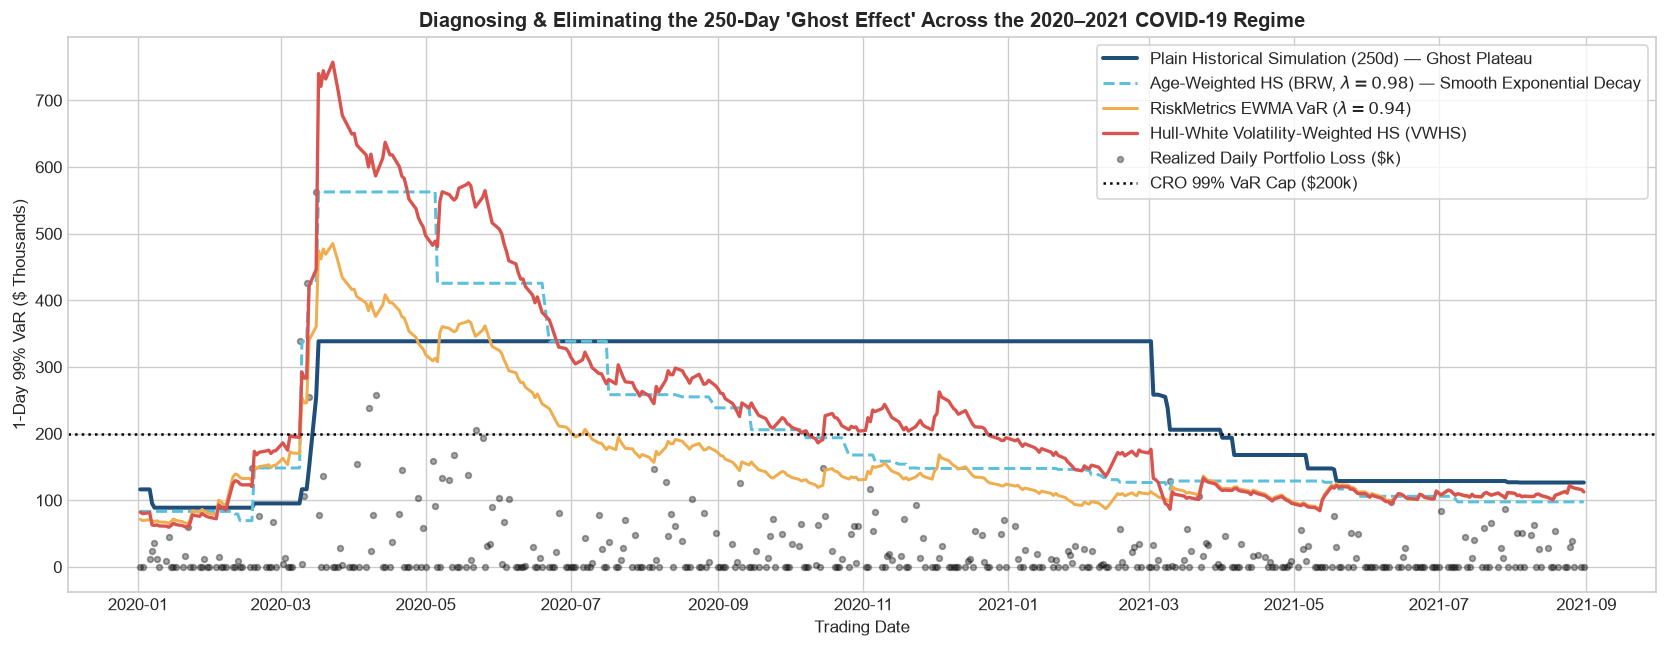
\includegraphics[width=0.98\textwidth]{figures/fig05_covid_ghost_effect.png}
\caption{Diagnosis and elimination of the 250-day ``Ghost Effect'' across the 2020--2021 COVID-19 regime, comparing Plain 250d HS against Age-Weighted HS ($\lambda=0.98$), RiskMetrics EWMA ($\lambda=0.94$), and Hull-White Volatility-Weighted HS.}
\end{figure}

To eliminate the ghost effect, \texttt{src/volatility\_models.py} implements four dynamic time-series estimators conditioned strictly on $\mathcal{F}_{t-1}$:
\begin{enumerate}
    \item \textbf{RiskMetrics EWMA Volatility ($\lambda = 0.94$, C++17 Kernel):}
    \begin{equation}
    \hat{\sigma}_{t \mid t-1}^2 = \lambda\hat{\sigma}_{t-1 \mid t-2}^2 + (1-\lambda)r_{p,t-1}^2
    \end{equation}
    \item \textbf{$\text{GARCH}(1,1)$ Conditional Volatility (Normal and Student-$t$ Innovations):}
    \begin{equation}
    r_{p,t} = \mu + \varepsilon_t, \qquad \hat{\sigma}_{t \mid t-1}^2 = \omega + \alpha_1\varepsilon_{t-1}^2 + \beta_1\hat{\sigma}_{t-1 \mid t-2}^2 \quad (\alpha_1 + \beta_1 < 1)
    \end{equation}
    Fitting $\text{GARCH}(1,1)$ on portfolio returns yields $\hat{\alpha}_1 = 0.0890, \hat{\beta}_1 = 0.8989$ (persistence $0.9879$) under Normal innovations ($\text{AIC} = 4,471.5$), and $\hat{\alpha}_1 = 0.0848, \hat{\beta}_1 = 0.9043$ (persistence $0.9892, \hat{\nu} = 7.34$) under Student-$t$ innovations ($\text{AIC} = 4,388.5$, improving log-likelihood by $+42.52$ points).
    \item \textbf{Age-Weighted Historical Simulation (BRW Hybrid, $\lambda_{\text{age}} = 0.98$):} Assigns exponential weights $w_i = \frac{\lambda_{\text{age}}^{i-1}(1-\lambda_{\text{age}})}{1-\lambda_{\text{age}}^n}$ to historical observations of age $i \in \{1, \dots, n\}$.
    \item \textbf{Hull-White (1998) Volatility-Weighted Historical Simulation (VWHS):} Rescales each historical return $r_{p,i}$ by the ratio of today's conditional volatility forecast $\hat{\sigma}_T$ to the historical volatility $\hat{\sigma}_i$ on day $i$:
    \begin{equation}
    r_{p,i}^* = r_{p,i}\left(\frac{\hat{\sigma}_T}{\hat{\sigma}_i}\right), \qquad L_i^* = -V_0 r_{p,i}^*
    \end{equation}
\end{enumerate}

Unlike Plain HS or Age-Weighted HS---which are bounded above by the maximum historical loss in the 250-day window---Hull-White VWHS forecasts 1-Day 99\% VaR strictly exceeding the worst unscaled loss in the 250-day window on 19 volatility-spike days (peaking at $\$785,221$ vs.\ $\$562,732$ unscaled window maximum in March 2020).

\begin{figure}[H]
\centering
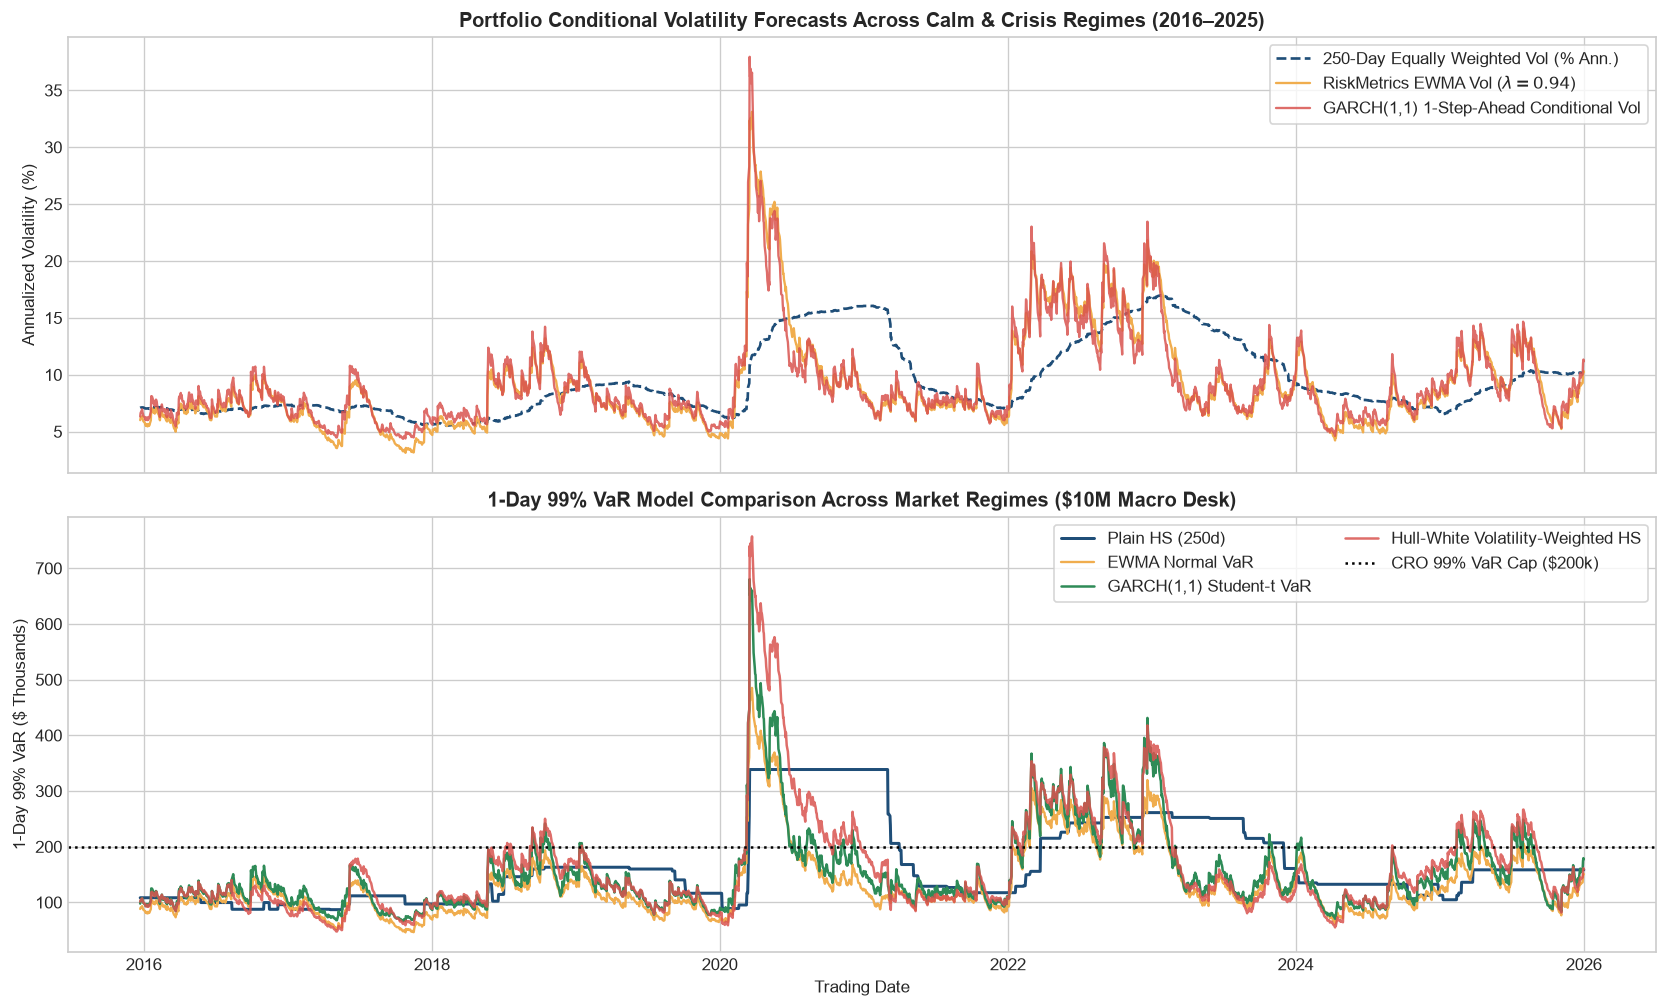
\includegraphics[width=0.98\textwidth]{figures/fig06_dynamic_var_regimes.png}
\caption{Top: Conditional annualized volatility forecasts (250d Rolling, RiskMetrics EWMA, and $\text{GARCH}(1,1)$) across 2016--2025. Bottom: Out-of-sample 1-Day 99\% VaR forecasts across calm and crisis regimes.}
\end{figure}

% ==============================================================================
\section{Phase 3 (Walk+): Out-of-Sample Statistical Backtesting and Champion--Challenger Validation}
% ==============================================================================

\subsection{Basel Traffic Light Framework, Kupiec POF and Christoffersen Markov Tests}

Over a $N = 1,500$-day out-of-sample window (2020--2025, expected 99\% breaches $= 15.0$), \texttt{src/backtesting.py} records the binary hit sequence $I_t = \mathbb{I}(L_t > \text{VaR}_{0.99, t \mid t-1})$ and evaluates three statistical validation criteria:
\begin{enumerate}
    \item \textbf{Basel Committee Traffic Light Zones (250-Day Rolling Window):} Classifies rolling 250-day 99\% breach counts $x_{250}$ into the \textbf{Green Zone ($0\text{--}4$ breaches, $+0.00$ capital add-on)}, \textbf{Yellow Zone ($5\text{--}9$ breaches, $+0.40$ to $+0.85$ penalty)}, and \textbf{Red Zone ($\ge 10$ breaches, $+1.00$ penalty and disqualification presumption)}.
    \item \textbf{Kupiec (1995) Proportion of Failures (POF) Test ($LR_{UC} \sim \chi^2_1$):} Tests unconditional coverage $\mathcal{H}_0: \pi = p = 1 - \alpha = 0.01$ with $x = \sum_{t=1}^N I_t$:
    \begin{equation}
    LR_{UC} = -2\ln\left(\frac{p^x(1-p)^{N-x}}{\left(\frac{x}{N}\right)^x\left(1-\frac{x}{N}\right)^{N-x}}\right) \xrightarrow{d} \chi^2_1 \quad (\text{5\% Critical Value} = 3.8415)
    \end{equation}
    \item \textbf{Christoffersen (1998) Markov Independence ($LR_{IND}$) and Conditional Coverage ($LR_{CC}$):} Counting adjacent-day transition states $(n_{00}, n_{01}, n_{10}, n_{11})$ with $\hat{\pi}_{01} = \frac{n_{01}}{n_{00}+n_{01}}$, $\hat{\pi}_{11} = \frac{n_{11}}{n_{10}+n_{11}}$, and $\hat{\pi} = \frac{n_{01}+n_{11}}{n_{00}+n_{01}+n_{10}+n_{11}}$:
    \begin{equation}
    LR_{IND} = -2\ln\left(\frac{(1-\hat{\pi})^{n_{00}+n_{10}}\hat{\pi}^{n_{01}+n_{11}}}{(1-\hat{\pi}_{01})^{n_{00}}\hat{\pi}_{01}^{n_{01}}(1-\hat{\pi}_{11})^{n_{10}}\hat{\pi}_{11}^{n_{11}}}\right) \xrightarrow{d} \chi^2_1, \qquad LR_{CC} = LR_{UC} + LR_{IND} \xrightarrow{d} \chi^2_2
    \end{equation}
    where $LR_{CC}$ rejects joint conditional coverage at the 5\% significance level if $LR_{CC} > 5.9915$.
\end{enumerate}

\subsection{Empirical Champion--Challenger Model Validation Results (1,500 Out-of-Sample Days)}

\begin{table}[H]
\centering
\caption{Champion--Challenger 1,500-Day Out-of-Sample Model Validation Table ($\alpha = 99\%$, Expected $= 15.0$)}
\scriptsize
\begin{tabular}{lrrrcrrrrl}
\toprule
\textbf{Model} & \textbf{Breaches} & \textbf{Rate} & \textbf{$n_{11}$} & \textbf{Latest / Peak Zone} & \textbf{$LR_{UC}$ ($p$)} & \textbf{$LR_{IND}$ ($p$)} & \textbf{$LR_{CC}$ ($p$)} & \textbf{Validation Verdict} \\
\midrule
Plain Historical Sim (250d) & 22 & 1.47\% & \textbf{2} & Green (4) / \textcolor{darkred}{\textbf{Red (10)}} & 2.885 (0.089) & \textcolor{darkred}{\textbf{4.209 (0.040)}} & \textcolor{darkred}{\textbf{7.093 (0.029)}} & \textcolor{darkred}{\textbf{FAIL Independence}} \\
Static Rolling Normal (250d) & 35 & 2.33\% & \textbf{4} & Yellow (6) / \textcolor{darkred}{\textbf{Red (17)}} & \textcolor{darkred}{\textbf{19.581 (0.000)}} & \textcolor{darkred}{\textbf{6.959 (0.008)}} & \textcolor{darkred}{\textbf{26.540 (0.000)}} & \textcolor{darkred}{\textbf{FAIL Coverage \& Ind}} \\
RiskMetrics EWMA Normal & 29 & 1.93\% & 0 & Green (4) / Yellow (9) & \textcolor{darkred}{\textbf{10.369 (0.001)}} & 1.144 (0.285) & \textcolor{darkred}{\textbf{11.513 (0.003)}} & \textcolor{darkred}{\textbf{FAIL Coverage}} \\
$\text{GARCH}(1,1)$ Normal & 33 & 2.20\% & 0 & Yellow (5) / Yellow (9) & \textcolor{darkred}{\textbf{16.257 (0.000)}} & 1.486 (0.223) & \textcolor{darkred}{\textbf{17.743 (0.000)}} & \textcolor{darkred}{\textbf{FAIL Coverage}} \\
\midrule
\textbf{$\text{GARCH}(1,1)$ Student-$t$ (FHS)} & \textbf{22} & \textbf{1.47\%} & \textbf{0} & \textcolor{darkgreen}{\textbf{Green (2)}} / Yellow (6) & \textbf{2.885 (0.089)} & \textbf{0.655 (0.418)} & \textbf{3.540 (0.170)} & \textcolor{darkgreen}{\textbf{PASS (Champion)}} \\
\textbf{Age-Weighted HS (BRW)} & \textbf{21} & \textbf{1.40\%} & \textbf{0} & \textcolor{darkgreen}{\textbf{Green (2)}} / Yellow (8) & \textbf{2.156 (0.142)} & \textbf{0.597 (0.440)} & \textbf{2.753 (0.252)} & \textcolor{darkgreen}{\textbf{PASS (Champion)}} \\
\textbf{Hull-White VWHS} & \textbf{18} & \textbf{1.20\%} & \textbf{0} & \textcolor{darkgreen}{\textbf{Green (1)}} / Yellow (6) & \textbf{0.570 (0.450)} & \textbf{0.438 (0.508)} & \textbf{1.007 (0.604)} & \textcolor{darkgreen}{\textbf{PASS (Best Overall)}} \\
\bottomrule
\end{tabular}
\end{table}

\begin{figure}[H]
\centering
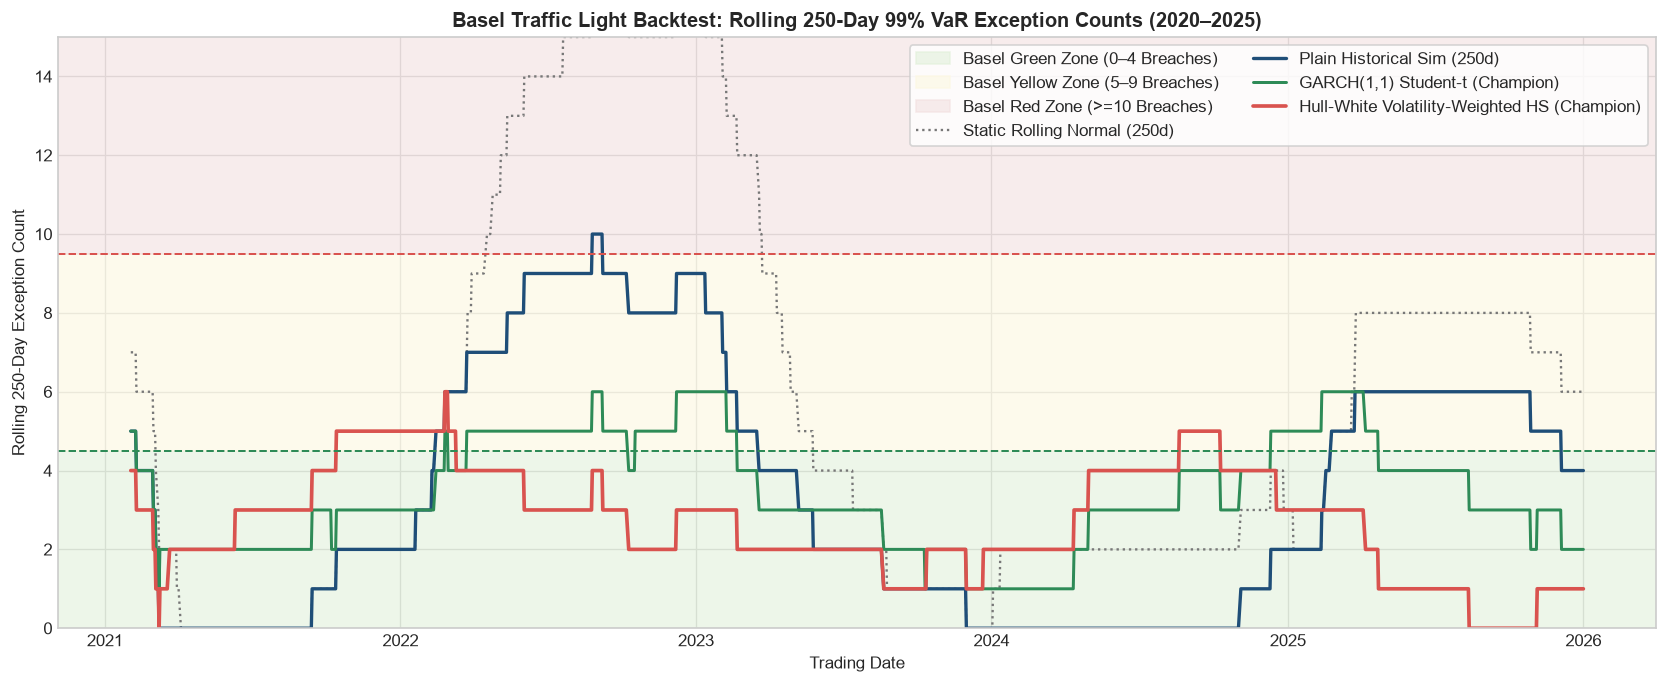
\includegraphics[width=0.96\textwidth]{figures/fig07_basel_traffic_light.png}
\caption{Basel Traffic Light rolling 250-day 99\% VaR exception counts across 2020--2025.}
\end{figure}

\begin{figure}[H]
\centering
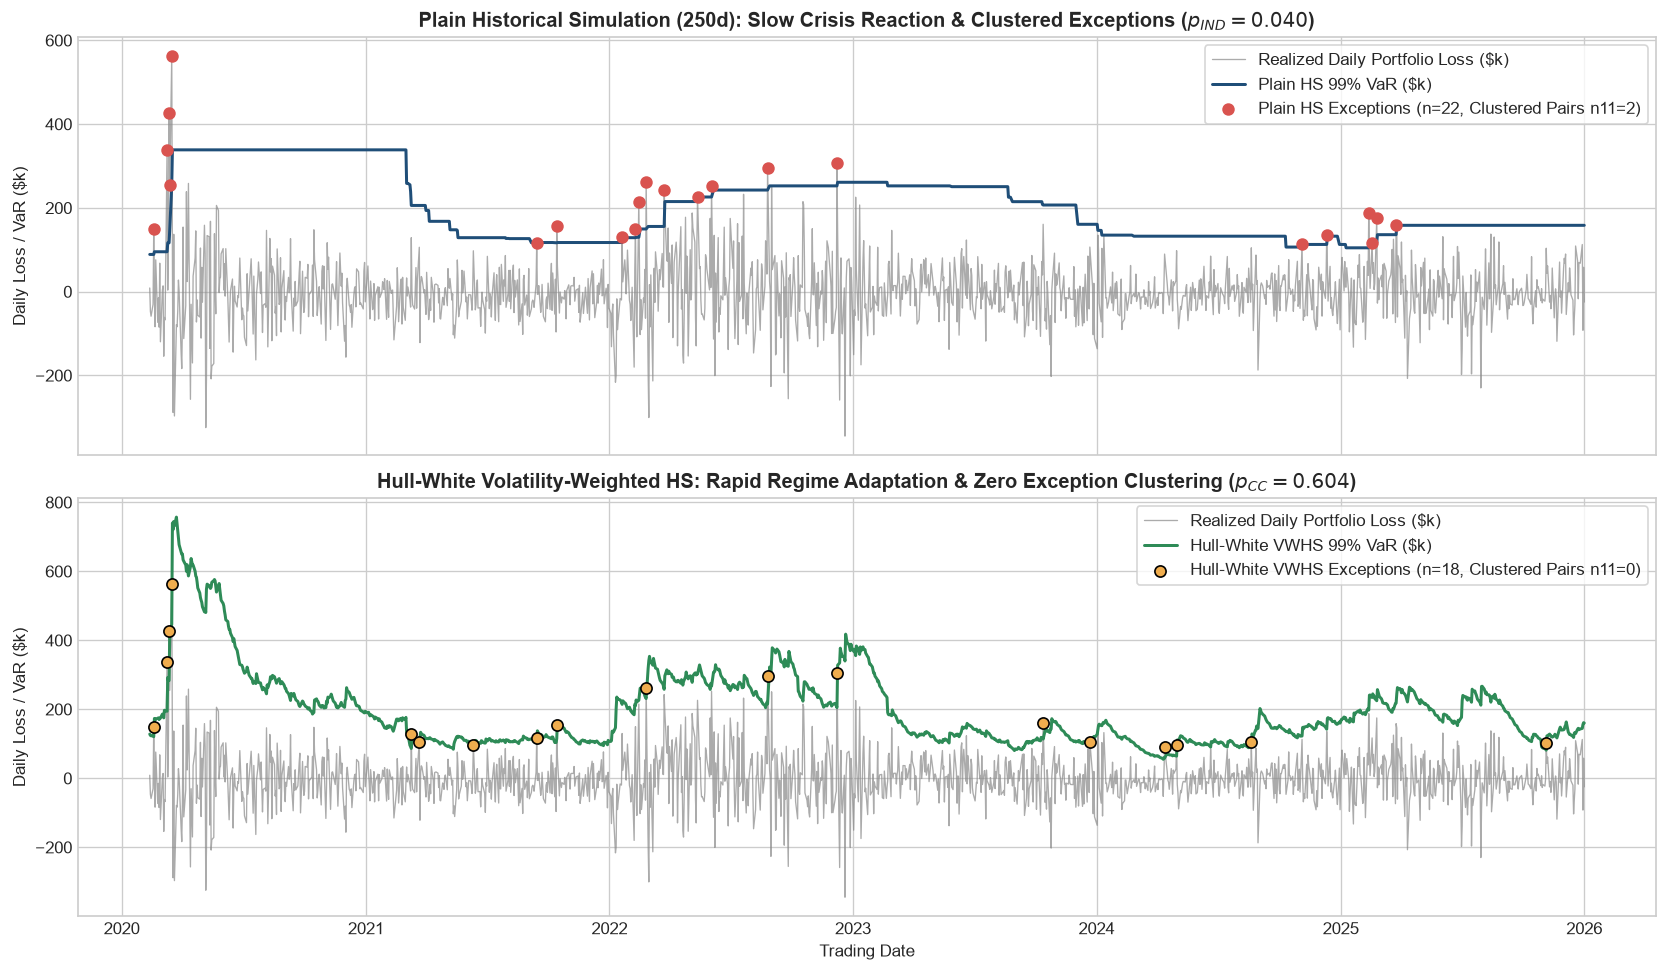
\includegraphics[width=0.96\textwidth]{figures/fig08_exception_clustering_timeline.png}
\caption{Out-of-sample 99\% VaR exception clustering timeline: Plain 250d Historical Simulation ($n=22, n_{11}=2, p_{IND}=0.040$) versus Hull-White Volatility-Weighted HS ($n=18, n_{11}=0, p_{CC}=0.604$).}
\end{figure}

Table 7 and Figures 7--8 prove the central empirical thesis of Phase 3: \textbf{Plain 250-day Historical Simulation passes Kupiec unconditional coverage ($p_{UC}=0.089$) only because its post-crisis ghost plateau suppresses breaches in calm years, but it fails Christoffersen Markov Independence ($n_{11}=2, p_{IND}=0.040$) and Joint Conditional Coverage ($p_{CC}=0.029$) due to consecutive breach clustering during crisis onset.} Conversely, dynamic Gaussian models (EWMA Normal and $\text{GARCH}(1,1)$ Normal) eliminate clustering ($n_{11}=0$) but fail Kupiec coverage ($p_{UC} \le 0.001$) due to thin normal tails. Only \textbf{Hull-White Volatility-Weighted HS} ($18$ breaches, $n_{11}=0, p_{CC}=0.604$), \textbf{$\text{GARCH}(1,1)$ Student-$t$} ($p_{CC}=0.170$), and \textbf{Age-Weighted HS} ($p_{CC}=0.252$) pass every regulatory and statistical test.

% ==============================================================================
\section{Phase 4 (Run): Non-Linear Derivative Portfolio Risk and Scenario Stress Testing}
% ==============================================================================

\subsection{Black-Scholes-Merton Pricing, Implied Volatility Inversion and Analytical Greeks}

In \texttt{src/cpp/quant\_core.cpp} and \texttt{src/derivatives\_stress.py}, European call ($C$) and put ($P$) options on \texttt{SPY} ($S_0 = \$500, r = 4.50\%, q = 1.30\%, T = 30/365$) are priced via the exact Black-Scholes-Merton (1973) equations:
\begin{equation}
C = S e^{-qT}\Phi(d_1) - K e^{-rT}\Phi(d_2), \qquad P = K e^{-rT}\Phi(-d_2) - S e^{-qT}\Phi(-d_1), \qquad d_{1,2} = \frac{\ln(S/K) + (r - q \pm \frac{1}{2}\sigma_{IV}^2)T}{\sigma_{IV}\sqrt{T}}
\end{equation}
with Implied Volatility $\sigma_{IV} = f^{-1}(P_{\text{mkt}}, S, K, r, T, q)$ inverted via a safeguarded Newton-Raphson / Brent-Bisection solver to a maximum inversion error of $5.34 \times 10^{-9}$, alongside closed-form analytical Greeks ($\Delta = \frac{\partial V}{\partial S}$, $\Gamma = \frac{\partial^2 V}{\partial S^2}$, $\mathcal{V} = \frac{\partial V}{\partial \sigma_{IV}}$, and $\Theta = \frac{\partial V}{\partial t}$).

\begin{figure}[H]
\centering
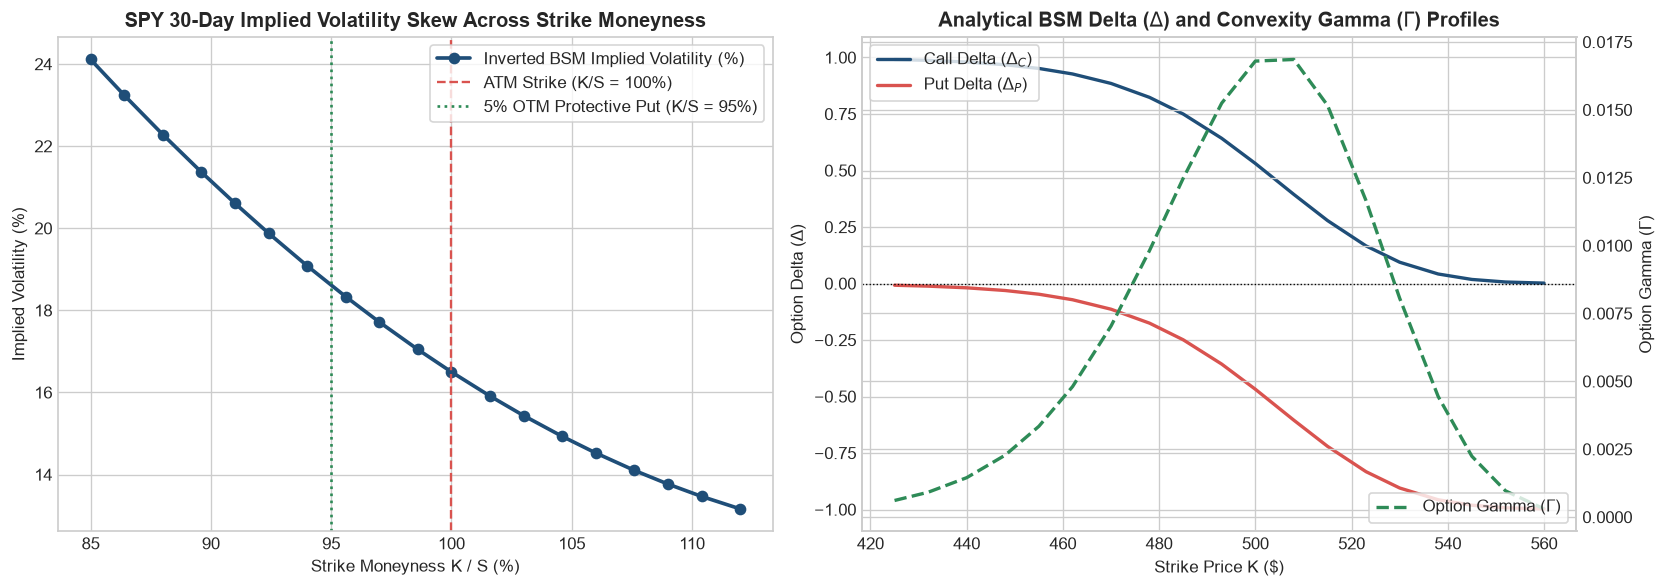
\includegraphics[width=0.98\textwidth]{figures/fig09_spy_iv_skew_and_greeks.png}
\caption{Left: Inverted 30-day \texttt{SPY} implied volatility skew across strike moneyness $K/S \in [85\%, 112\%]$. Right: Analytical BSM call/put Delta ($\Delta$) and convexity Gamma ($\Gamma$) profiles.}
\end{figure}

\subsection{Comparing Derivative VaR Engines: Delta-Normal vs.\ Delta-Gamma-Vega vs.\ Full Revaluation MC}

Across $M = 20,000$ correlated Monte Carlo scenarios of daily \texttt{SPY} spot returns ($\sigma_S = 1.10\%$) and implied volatility shocks ($\sigma_{\Delta IV} = 1.45\text{ vol pts}, \rho_{S,IV} = -0.72$), we compare:
\begin{align}
\Delta V_{\text{Delta-Normal}} &\approx \Delta_{\text{net}}\,\Delta S \\
\Delta V_{\text{DGV}} &\approx \Delta_{\text{net}}\,\Delta S + \frac{1}{2}\Gamma_{\text{net}}(\Delta S)^2 + \mathcal{V}_{\text{net}}\,\Delta\sigma_{IV} + \Theta_{\text{net}}\,\Delta t \\
\Delta V_{\text{Full MC}}^{(m)} &= \sum_j n_j \left[V_{\text{BSM}, j}(S_{t+1}^{(m)}, \sigma_{IV, j, t+1}^{(m)}, T-\Delta t) - V_{\text{BSM}, j}(S_t, \sigma_{IV, j, t}, T)\right]
\end{align}

\begin{table}[H]
\centering
\caption{1-Day 99\% Derivative VaR and ES Comparison ($M = 20,000$ Scenarios, \texttt{04\_derivatives\_and\_stress\_testing.ipynb})}
\scriptsize
\begin{tabular}{lrrrrrrr}
\toprule
\textbf{Option Portfolio Structure} & \textbf{$\Delta_{\text{net}}$ (sh)} & \textbf{\$ Gamma} & \textbf{Vega/1\%} & \textbf{Delta-Norm VaR} & \textbf{DGV VaR} & \textbf{Full MC VaR} & \textbf{Full MC ES} \\
\midrule
Long Delta-Neutral Straddle (+6,000 sh) & \textbf{0.00} & +\$2,527.37 & +\$6,855.06 & \textcolor{darkred}{\textbf{\$0.00}} & \$20,131.40 & \textbf{\$19,320.09} & \$21,564.56 \\
Short Delta-Neutral Straddle ($-6,000$ sh) & \textbf{0.00} & $-\$2,527.37$ & $-\$6,855.06$ & \textcolor{darkred}{\textbf{\$0.00}} & \$34,184.63 & \textbf{\$31,305.43} & \textbf{\$38,162.12} \\
Hedged \$3M \texttt{SPY} + 5\% OTM Put & +5,095.63 & +\$654.23 & +\$2,011.09 & \textbf{\$65,198.20} & \$58,004.57 & \textbf{\$55,893.34} & \$62,292.02 \\
\bottomrule
\end{tabular}
\end{table}

\begin{figure}[H]
\centering
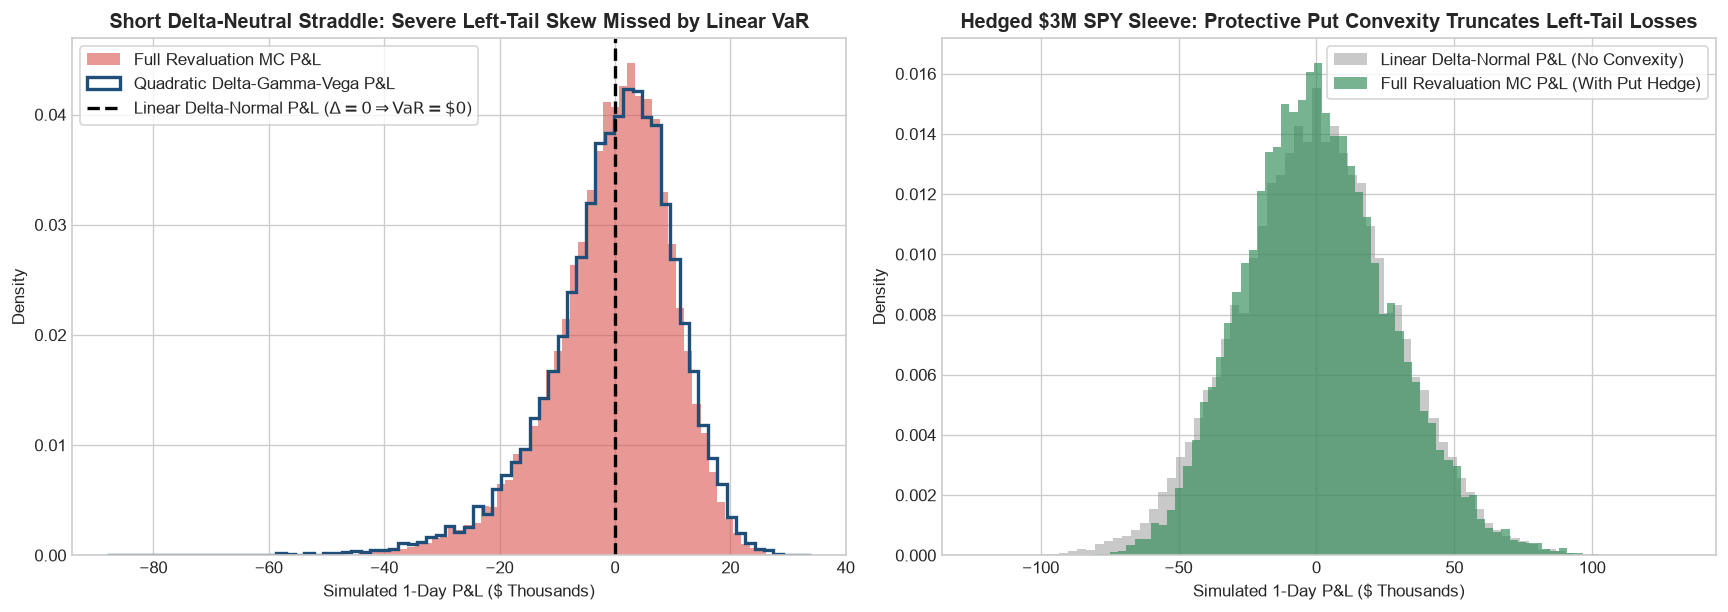
\includegraphics[width=0.98\textwidth]{figures/fig10_straddle_and_hedged_pnl_dists.png}
\caption{Left: Short Delta-Neutral Straddle P\&L distribution showing severe negative-gamma / short-vega tail losses completely missed by Linear Delta-Normal VaR ($\Delta=0 \implies \text{VaR}=\$0$). Right: Hedged \$3M \texttt{SPY} sleeve showing left-tail loss truncation from positive put convexity.}
\end{figure}

As shown in Table 8 and Figure 10, on a \textbf{Short Delta-Neutral Straddle} ($\Delta_{\text{net}} = 0.00$), \textbf{Linear Delta-Normal VaR reports exactly \$0.00 of risk}, missing \textbf{\$31,305.43 in Full Revaluation 99\% VaR} (\textbf{\$38,162.12 in 99\% ES}) driven by negative convexity ($\Gamma < 0$) and short vega ($\mathcal{V} < 0$). Conversely, on the \textbf{Hedged \$3M \texttt{SPY} + 5\% OTM Protective Put} book, Delta-Normal VaR overstates 99\% VaR by \textbf{+\$9,304.85 (+16.6\%)} because it ignores the protective put's positive convexity cushion.

\subsection{Historical Crisis Replay and 2D Hypothetical Spot--Volatility Stress Grids}

Replaying the exact historical daily returns and VIX shocks of the \textbf{2020 COVID-19 Crash} (Feb 19 -- Mar 31, 2020) shows that hedging the \$3M \texttt{SPY} sleeve with a 5\% OTM protective put generates \textbf{+\$370,616.60 in put hedge gains}, turning an unhedged cumulative drawdown of $-\$308,745.74$ into a net $+\$61,870.86$ gain and cutting the worst single-day crash loss by \textbf{33.04\%} (from $-\$562,732.26$ to $-\$376,817.11$). Across the $5 \times 5$ hypothetical Spot $\times$ Implied Volatility stress grid (Figure 11), in the extreme \textbf{\texttt{Spot -20\%, IV +25 pts}} cell, the protective put reduces total desk losses from $-\$930,000$ (unhedged) to $-\$487,511$ (\textbf{saving \$442,489, or 47.6\%}), while retaining \textbf{97.3\% of bull-market upside} ($+\$452,249$ vs.\ $+\$465,000$) in the \texttt{Spot +10\%, IV +0 pts} rally scenario.

\begin{figure}[H]
\centering
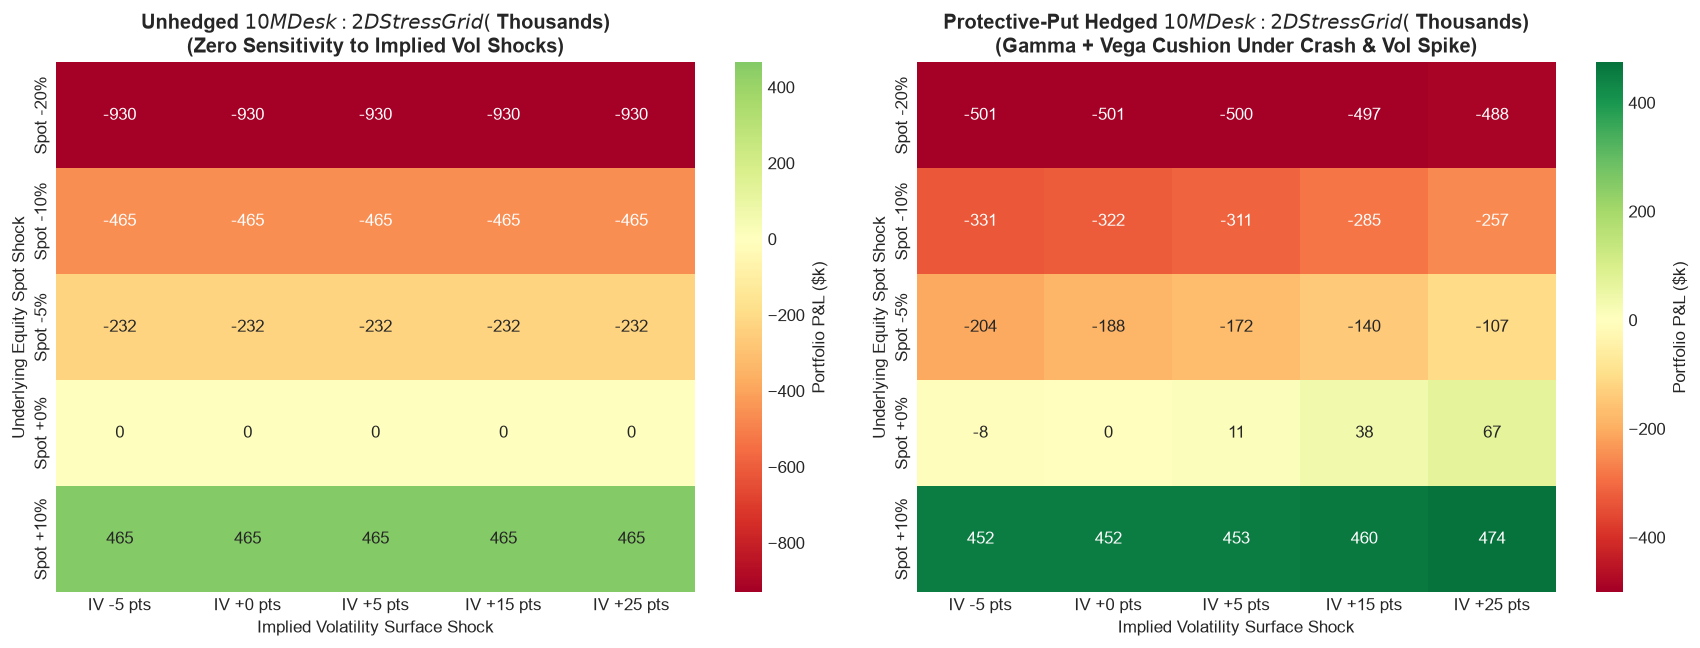
\includegraphics[width=0.98\textwidth]{figures/fig11_2d_stress_vulnerability_heatmaps.png}
\caption{2D Hypothetical Stress Vulnerability Grid ($5\times 5$ Spot $\times$ Implied Volatility shock matrix) comparing the Unhedged \$10M Desk (left) against the Protective-Put Hedged \$10M Desk (right).}
\end{figure}

% ==============================================================================
\section{Synthesis of Model Governance Recommendations and References}
% ==============================================================================

\begin{enumerate}
    \item \textbf{Production Linear VaR/ES Champion Model:} Deploy \textbf{Hull-White (1998) Volatility-Weighted Historical Simulation} (backed by \textbf{$\text{GARCH}(1,1)$ Student-$t$ FHS}) for daily CRO limit monitoring. Both models eliminate the 250-day ghost plateau and pass Kupiec POF and Christoffersen Markov Independence tests ($n_{11}=0, p_{CC}=0.604$ and $0.170$) in the Basel Green Zone.
    \item \textbf{Pre-Trade Limit Sizing:} Use exact numerical root-finding (\texttt{brentq}) rather than linear Marginal VaR approximations when sizing volatile additions (\texttt{TSLA} capped at \$765.2k HS / \$961.3k Normal under the \$200k CRO limit).
    \item \textbf{Derivatives Risk Engine:} Mandate \textbf{C++17 Full Revaluation Monte Carlo} and $5\times 5$ Spot--Volatility stress grids for all option positions, prohibiting linear Delta-Normal VaR on non-linear portfolios.
\end{enumerate}

\begingroup
\renewcommand{\section}[2]{}
\small
\begin{thebibliography}{99}
\bibitem{acerbi2002} Acerbi, C., and Tasche, D. (2002). On the Coherence of Expected Shortfall. \textit{Journal of Banking \& Finance}, 26(7), 1487--1503.
\bibitem{artzner1999} Artzner, P., Delbaen, F., Eber, J.-M., and Heath, D. (1999). Coherent Measures of Risk. \textit{Mathematical Finance}, 9(3), 203--228.
\bibitem{bcbs1996} Basel Committee on Banking Supervision (1996). \textit{Supervisory Framework for the Use of ``Backtesting'' in Conjunction with the Internal Models Approach to Market Risk Capital Requirements}. BIS.
\bibitem{bcbs2019} Basel Committee on Banking Supervision (2019). \textit{Minimum Capital Requirements for Market Risk (FRTB)}. BIS d457.
\bibitem{bs1973} Black, F., and Scholes, M. (1973). The Pricing of Options and Corporate Liabilities. \textit{Journal of Political Economy}, 81(3), 637--654.
\bibitem{bollerslev1986} Bollerslev, T. (1986). Generalized Autoregressive Conditional Heteroskedasticity. \textit{Journal of Econometrics}, 31(3), 307--327.
\bibitem{brw1998} Boudoukh, J., Richardson, M., and Whitelaw, R. F. (1998). The Best of Both Worlds: A Hybrid Approach to Calculating Value at Risk. \textit{Risk}, 11(5), 64--67.
\bibitem{christoffersen1998} Christoffersen, P. F. (1998). Evaluating Interval Forecasts. \textit{International Economic Review}, 39(4), 841--862.
\bibitem{cf1938} Cornish, E. A., and Fisher, R. A. (1938). Moments and Cumulants in the Specification of Distributions. \textit{Revue de l'Institut International de Statistique}, 5(4), 307--320.
\bibitem{df1979} Dickey, D. A., and Fuller, W. A. (1979). Distribution of the Estimators for Autoregressive Time Series with a Unit Root. \textit{JASA}, 74(366a), 427--431.
\bibitem{hw1998} Hull, J., and White, A. (1998). Incorporating Volatility Updating into the Historical Simulation Method for Value-at-Risk. \textit{Journal of Risk}, 1(1), 5--19.
\bibitem{kupiec1995} Kupiec, P. H. (1995). Techniques for Verifying the Accuracy of Risk Measurement Models. \textit{Journal of Derivatives}, 3(2), 73--84.
\end{thebibliography}
\endgroup

\end{document}
